\documentclass{article}
\usepackage{xeCJK}
\usepackage{amsmath}
\usepackage{listings}
\usepackage{xcolor}
\setlength{\parindent}{0pt}
\renewcommand{\baselinestretch}{1.0}
\lstset{
	frame=tb, % draw a frame at the top and bottom of the code block
	showstringspaces=false, % don't mark spaces in strings
	numbers=left, % display line numbers on the left
	commentstyle=\color{green}, % comment color
	keywordstyle=\color{blue}, % keyword color
	stringstyle=\color{red} % string color
}
\usepackage[a4paper,left=20mm,right=20mm,top=15mm,bottom=15mm]{geometry}  

\title{gawk}
\author{MengChunlei}

\linespread{1.2}
\begin{document}
\maketitle
gawk是一个文本处理工具。它用起来更加接近高级编程语言。它的基本格式为: gawk script file.其中script是一段脚本程序,要放在单引号中。本文将按照以下7个部分来总结它的用法: \par
\begin{itemize}
	\item 基本用法
	\item 变量
	\item 数组
	\item 模式
    \item 控制逻辑
	\item 格式化打印
	\item 函数
\end{itemize}

\section{基本用法}
\subsection{提取字段}
\begin{itemize}
	\item \$0: 整个文本
	\item \$1: 本文中第一个字段
	\item \$n: 文本中第n个字段
\end{itemize}

\begin{lstlisting}[language=bash, caption={1.1}]
mcl@mcl$ cat file1 
data11 data12 data13
data21 data22 data23
data31 data32 data33
mcl@mcl$ gawk '{print $1, $3}' file1 /*默认用空格分割*/
data11 data13
data21 data23
data31 data33
mcl@mcl$ gawk '{print "The data is: " $1, $3}' file1 
The data is: data11 data13
The data is: data21 data23
The data is: data31 data33
\end{lstlisting}

\subsection{替换字段}
\begin{lstlisting}[language=bash, caption={1.2}]
mcl@mcl$ gawk '{$3="hello"; print "The data is: " $1, $3}' file1 
The data is: data11 hello
The data is: data21 hello
The data is: data31 hello
mcl@mcl$ echo "My name is alice" | gawk '{$4="mcl"; print $0}'
My name is mcl
mcl@mcl$ echo "My name is alice" | gawk '{  /*多个命令可以直接换行*/
> $4="mcl"
> print $0}'
My name is mcl
\end{lstlisting}

\subsection{从文件读取命令}
\begin{lstlisting}[language=bash, caption={1.3}]
mcl@mcl$ cat script1.gawk  /*将脚本存储在文件。同时可以看到可以用变量text*/
{
text = "'s home is: "
print $1 text $6
}
mcl@mcl$ gawk -F: -f script1.gawk /etc/passwd  /*-F可以设置分隔符*/
root's home is: /root
daemon's home is: /usr/sbin
bin's home is: /bin
sys's home is: /dev
sync's home is: /bin
games's home is: /usr/games
\end{lstlisting}

\subsection{数据处理前后运行脚本}
\begin{lstlisting}[language=bash, caption={1.4}]
mcl@mcl$ cat script2.gawk 
BEGIN {                   /*BEGIN定义了数据处理前运行的一段脚本,只运行一次*/
print "The passwd info:"
FS=":"              /*注意这里可以用FS设置分隔符*/
}
{
text = "'s home is: "
print $1 text $6
}
END{print "Data process finished"}  /*END定义了处理完后运行的脚本*/
mcl@mcl$ gawk -f script2.gawk /etc/passwd
The passwd info:
root's home is: /root
daemon's home is: /usr/sbin
bin's home is: /bin
Data process finished
\end{lstlisting}

\section{变量}
\subsection{输入输出字段分隔符}
\begin{lstlisting}[language=bash, caption={2.1}]
mcl@mcl$ cat file2
data11,data12,data13
data21,data22,data23
data31,data32,data33
mcl@mcl$ gawk 'BEGIN{FS=","} {print $1, $2, $3}' file2
data11 data12 data13
data21 data22 data23
data31 data32 data33
mcl@mcl$ gawk 'BEGIN{FS=","; OFS="-"} {print $1, $2, $3}' file2 
data11-data12-data13 /*OFS可以设置输出的分隔符,默认是空格*/
data21-data22-data23
data31-data32-data33
\end{lstlisting}
\subsection{按照宽度分割}
\begin{lstlisting}[language=bash, caption={2.2}]
mcl@mcl$ cat file3
1234557890
3234557867
2929817231
mcl@mcl$ gawk 'BEGIN{FIELDWIDTHS="3 4 3"} {print $1, $2, $3}' file3
123 4557 890   /*FIELDWIDTHS决定了各个字段的宽度*/
323 4557 867
292 9817 231
\end{lstlisting}
\subsection{输入输出记录分隔符}
\begin{lstlisting}[language=bash, caption={2.3}]
mcl@mcl$ cat file4
xiaoming
qinghua
18810101010

xiaobai
renda
18812345678
mcl@mcl$ gawk 'BEGIN{FS="\n"; RS=""} {print $1, $3}' file4 /*换行为字段分隔符*/
xiaoming 18810101010                    /*空行为记录分隔符*/
xiaobai 18812345678               /*默认输出记录分隔符为换行*/
mcl@mcl$ gawk 'BEGIN{FS="\n"; RS=""; ORS="\n====================\n"} {print $1, $3}' file4
xiaoming 18810101010     /*设定输出记录分隔符*/
====================
xiaobai 18812345678
====================
\end{lstlisting}
\subsection{其他内置变量}
\begin{lstlisting}[language=bash, caption={2.4}]
mcl@mcl$ gawk 'BEGIN{print ARGC, ARGV[0], ARGV[1]}' file4  /*打印参数个数和参数*/
2 gawk file4
mcl@mcl$ gawk 'BEGIN{print ENVIRON["PATH"]}' file4   /*打印环境变量*/
/opt/ros/melodic/bin:/usr/local/sbin:/usr/local/bin:/usr/sbin
mcl@mcl$ cat file2
data11,data12,data13
data21,data22,data23
data31,data32,data33
mcl@mcl$ gawk 'BEGIN{FS=","} {print $NF}' file2  /*NF代表了总的字段个数*/
data13
data23
data33
mcl@mcl$ gawk '
BEGIN {FS=""}
{print $1, "FNR="FNR, "NR="NR}
END{print "The total records: "NR}' file2 file2 /*注意这里文件被处理了两次*/
d FNR=1 NR=1    /*FNR表示当前文件已经处理的记录个数*/
d FNR=2 NR=2    /*NR表示当前命令已经处理的记录个数*/
d FNR=3 NR=3
d FNR=1 NR=4
d FNR=2 NR=5
d FNR=3 NR=6
The total records: 6
\end{lstlisting}
\subsection{自定义变量}
\begin{lstlisting}[language=bash, caption={2.5}]
mcl@mcl$ gawk 'BEGIN {   /*设置变量;变量可以被改变; 可以进行数学运算*/
text="this is test"; print text
text=1209; test=text*2
print text}'
this is test
1209
mcl@mcl$ cat script3.gawk 
BEGIN{FS=","; print "the n=", n}
{print $n}
mcl@mcl$ gawk -f script3.gawk n=3 file2  /*设置的n=3对 BEGIN无效*/
the n= 
data13
data23
data33
mcl@mcl$ gawk -v n=3 -f script3.gawk file2 /*BEGIN中的变量需要用-v设置*/
the n= 3
data13
data23
data33
\end{lstlisting}

\section{数组}
\subsection{数组定义}
\begin{lstlisting}[language=bash, caption={3.1}]
mcl@mcl$ gawk 'BEGIN{
mapper["data11"]=100
mapper["data21"]=2000
mapper["data31"]=30000
}
{print mapper[$1]}' file1
100
2000
30000
\end{lstlisting}
\subsection{数组遍历和删除}
\begin{lstlisting}[language=bash, caption={3.2}]
mcl@mcl$ gawk 'BEGIN{
mapper["data11"]=100
mapper["data12"]=2000
mapper["data31"]=30000
for (e in mapper) {
  print "key: ", e, " -> ", mapper[e]
}
}'
key:  data11  ->  100
key:  data12  ->  2000
key:  data31  ->  30000
mcl@mcl$ gawk 'BEGIN{
mapper["data11"]=100
mapper["data12"]=2000
mapper["data31"]=30000
for (e in mapper) {
  print "key: ", e, " -> ", mapper[e]
}
delete mapper["data12"]
print "===="
for (e in mapper) {
  print "key: ", e, " -> ", mapper[e]
}
}'
key:  data11  ->  100
key:  data12  ->  2000
key:  data31  ->  30000
====
key:  data11  ->  100
key:  data31  ->  30000
\end{lstlisting}

\section{模式}

\subsection{正则表达式}
\begin{lstlisting}[language=bash, caption={4.1}]
mcl@mcl$ cat file2
data11,data12,data13
data21,data22,data23
data31,data32,data33
mcl@mcl$ gawk '/22/{print $0}' file2  /*包含22的行会被处理*/
data21,data22,data23
\end{lstlisting}\subsection{匹配符}
\begin{lstlisting}[language=bash, caption={4.2}]
mcl@mcl$ gawk 'BEGIN{FS=","} $2 ~ /data[2,3]/{print $0}' file2
data21,data22,data23                    /*第二个字段包含data2或者data3*/
data31,data32,data33
mcl@mcl$ 
mcl@mcl$ gawk 'BEGIN{FS=","} $2 !~ /data[2,3]/{print $0}' file2
data11,data12,data13                    /*第二个字段不包含data2或者data3*/
\end{lstlisting}
\subsection{数学表达式}
\begin{lstlisting}[language=bash, caption={4.3}]
mcl@mcl$ cat file3
1234557890
3234557867
2929817231
mcl@mcl$ gawk 'BEGIN{FIELDWIDTHS="3 4 3"} $1 < 300{print $1, $2, $3}' file3
123 4557 890
292 9817 231
\end{lstlisting}

\section{控制逻辑}

\subsection{if}
\begin{lstlisting}[language=bash, caption={5.1}]
mcl@mcl$ cat file5
23
19
15
mcl@mcl$ cat script4.gawk 
{
if ($1 > 20) {
  print $1 * 2
} else {
  print $1 + 10
}
}
mcl@mcl$ gawk -f script4.gawk file5
46
29
25
\end{lstlisting}
\subsection{while}
\begin{lstlisting}[language=bash, caption={5.2}]
mcl@mcl$ cat file6
12 3 10 5
9 12
4 6 30
mcl@mcl$ cat script5.gawk 
{
total = 0
i = 1
while (i <= NF) {
  total += $i
  ++i
}
avg = total / NF
print "average is:", total, "/", NF, "=", avg
}
mcl@mcl$ gawk -f script5.gawk file6
average is: 30 / 4 = 7.5
average is: 21 / 2 = 10.5
average is: 40 / 3 = 13.3333
\end{lstlisting}
\subsection{for}
\begin{lstlisting}[language=bash, caption={5.3}]
mcl@mcl$ cat script6.gawk 
{
total = 0
for (i = 1; i <= NF; ++i) {
  total += $i
}
avg = total / NF
print "average is:", total, "/", NF, "=", avg
}
mcl@mcl$ gawk -f script6.gawk file6
average is: 30 / 4 = 7.5
average is: 21 / 2 = 10.5
average is: 40 / 3 = 13.3333
\end{lstlisting}

\section{格式化打印}
\subsection{各种类型}
\begin{lstlisting}[language=bash, caption={6.1}]
mcl@mcl$ cat script7.gawk 
BEGIN{
x = 75
printf "  ascii: %c\n", x
printf "integer: %d\n", x
printf "      e: %e\n", x
printf "  float: %f\n", x
printf "  octal: %o\n", x
printf "    hex: %x\n", x
printf "    HEX: %X\n", x
}
mcl@mcl$ gawk -f script7.gawk 
  ascii: K
integer: 75
   e: 7.500000e+01
 float: 75.000000
 octal: 113
  hex: 4b
  HEX: 4B
\end{lstlisting}
\subsection{对齐和宽度}
\begin{lstlisting}[language=bash, caption={6.2}]
mcl@mcl$ cat file7
zhangsan 19801212 93.45
lisi 19900916 88.5
wangwu 20050304 70.123
mcl@mcl$ gawk '{printf "%9s %s %.5f\n", $1, $2, $3}' file7
 zhangsan 19801212 93.45000   /*靠右对齐*/
     lisi 19900916 88.50000
   wangwu 20050304 70.12300
mcl@mcl$ gawk '{printf "%-9s %s %.5f\n", $1, $2, $3}' file7
zhangsan  19801212 93.45000    /*靠左对齐*/
lisi      19900916 88.50000
wangwu    20050304 70.12300
\end{lstlisting}

\section{函数}
\subsection{数学函数}
\begin{lstlisting}[language=bash, caption={7.1}]
mcl@mcl$ cat script8.gawk 
BEGIN{
pi = 3.1415926
printf "    sin(30): %.4f\n", sin(pi / 6)
printf "    cos(30): %.4f\n", cos(pi / 6)
printf "     exp(2): %.4f\n", exp(2)
printf "    int(pi): %.4f\n", int(pi)
printf "log(exp(2)): %.4f\n", log(exp(2))
printf "     rand(): %.4f\n", rand()  /*rand返回的是[0,1]之间的小数*/
printf "     rand(): %.4f\n", rand()
printf "    sqrt(9): %.4f\n", sqrt(9)
printf "   and(5,6): %d\n", and(5, 6)
printf "    or(5,6): %d\n", or(5, 6)
printf "   xor(5,6): %d\n", xor(5, 6)
printf "lshift(5,2): %d\n", lshift(5,2)
printf "rshift(5,2): %d\n", rshift(5,2)
}
mcl@mcl$ gawk -f script8.gawk 
    sin(30): 0.5000
    cos(30): 0.8660
     exp(2): 7.3891
    int(pi): 3.0000
log(exp(2)): 2.0000
     rand(): 0.2378
     rand(): 0.2911
    sqrt(9): 3.0000
   and(5,6): 4
    or(5,6): 7
   xor(5,6): 3
lshift(5,2): 20
rshift(5,2): 1
\end{lstlisting}
\subsection{字符串函数}
\begin{lstlisting}[language=bash, caption={7.2}]
mcl@mcl$ cat script9.gawk 
BEGIN{
s="11, abc, 11, pqr"
printf "          gensub: %s\n", gensub("11", "22", 1, s) /*替换第一次11*/
printf "          gensub: %s\n", gensub("11", "22", 2, s)
printf "          gensub: %s\n", gensub("11", "22", "g", s) /*替换所有11*/
printf "          gensub: %s\n", gensub("a[a-z]{2}", "xxx", "g", s) /*支持正则表达式*/
printf "gsub-replace-num: %d\n", gsub("11", "22", s) /*将所有11替换,返回替换的个数*/
printf " replace-by-gsub: %s\n", s  /*s被改变*/
s="11, abc, 11, pqr"
printf "           index: %d\n", index(s, "abc") /*返回第一次出现的位置,下标从1开始*/
printf "           index: %d\n", index(s, "xxx") /*没有找到返回0*/
printf "          length: %d\n", length(s)
printf "           match: %d\n", match("xx11,11", "11") /*返回第一次match的起始位置*/
printf "           match: %d\n", match("xx11,11", "11", a)
for (x in a) {  /*数组a中保存了第一次匹配的位置和长度*/
print x, " -> ", a[x]
}
printf "           split: %d\n", split("xx11,11,1323", b, ",") /*将逗号分隔的结果放到b*/
for (x in b) {
print x, " -> ", b[x]
}
printf "         sprintf: %s\n", sprintf("format data: [%s], %d", s, 123)
printf "          substr: %s\n", substr(s, 5, 3)
printf "         toupper: %s\n", toupper("abc")
printf "         tolower: %s\n", tolower("abcDEF")
}
\end{lstlisting}
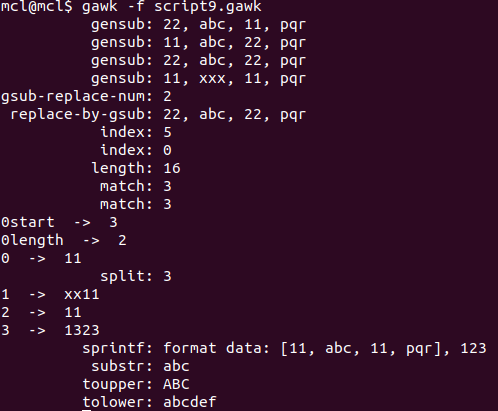
\includegraphics[scale=0.8]{pic1.png} \par
\subsection{时间函数}
\begin{lstlisting}[language=bash, caption={7.3}]
mcl@mcl$ cat script10.gawk 
BEGIN{
date = systime()
day = strftime("%A, %b %d, %Y", date)
print day
tp = mktime("2021 03 27 12 58 30")
print tp
print strftime("%A, %b %d, %Y", tp)
}
mcl@mcl$ gawk -f script10.gawk 
星期六, 3月 27, 2021
1616821110
星期六, 3月 27, 2021
\end{lstlisting}
\subsection{自定义函数}
\begin{lstlisting}[language=bash, caption={7.4}]
mcl@mcl$ cat  script11.gawk
function myprint(a, b, c) {
  printf "%10s %d %.5f\n", a, b, c 
}
{
myprint($1, $2, $3)
}
mcl@mcl$ gawk -f script11.gawk file7
zhangsan 19801212 93.45000
    lisi 19900916 88.50000
  wangwu 20050304 70.12300
\end{lstlisting}
\subsection{函数库}
\begin{lstlisting}[language=bash, caption={7.5}]
mcl@mcl$ cat funclib.gawk 
function print2(a, b) {
  printf "%10s %d", a, b
}

function print_third() {
  printf " %.4f\n", $3
}

mcl@mcl$ cat script12.gawk 
{
print2($1, $2)
print_third()
}
mcl@mcl$ gawk -f funclib.gawk -f script12.gawk file7
zhangsan 19801212 93.4500
    lisi 19900916 88.5000
  wangwu 20050304 70.1230
\end{lstlisting}
\end{document}

